
\documentclass{beamer}

% official, as per http://www.uvm.edu/~mmetivie/?Page=rules_logo.html
% Green: R:0 G:104 B:71
% white: R:255 G:250 B:250 

\definecolor{green}{RGB}{0,104,71}
\definecolor{white}{RGB}{255,250,250}

\usepackage{gensymb}

\usepackage{graphicx}
\graphicspath{{./img/}}

\mode<presentation>
{
  \usetheme{default}
  \setbeamertemplate{navigation symbols}{}
  \setbeamercolor{titlelike}{fg=white,bg=green}
  \useinnertheme[shadow=true]{rounded}
  \setbeamercolor{item projected}{fg=green,bg=green!20}
  \setbeamertemplate{blocks}[rounded][shadow=true]
}

\title[]{Ecological Genomics of the \textit{Climate Cascade}}

\author{John Stanton-Geddes}

\institute{Department of Biology \\ University of Vermont}

\setlength{\parskip}{14.0pt plus 8.0pt minus 3.0pt}

\begin{document}

\begin{frame}
  \titlepage
\end{frame}


\begin{frame}{Overview}
  \begin{enumerate}
  	\item<1->Progress on the \textit{Aphaenogaster} transcriptome
  	\item<2-> Identifying genes associated with thermal tolerance
	\item<3-> Latitudinal variation in gene expression
  	\item<4-> Population genomics of \textit{Aphaenogaster}
  	\item<5-> What is the adaptive potential of \textit{Aphaenogaster} to climate change?
  \end{enumerate}
\end{frame}

\begin{frame}{}
	\huge\begin{quote}
		Why am I here?
	\end{quote}
	\normalsize
\end{frame}


\begin{frame}{Species range limits}
	\begin{columns}
		 \begin{column}{5cm}
			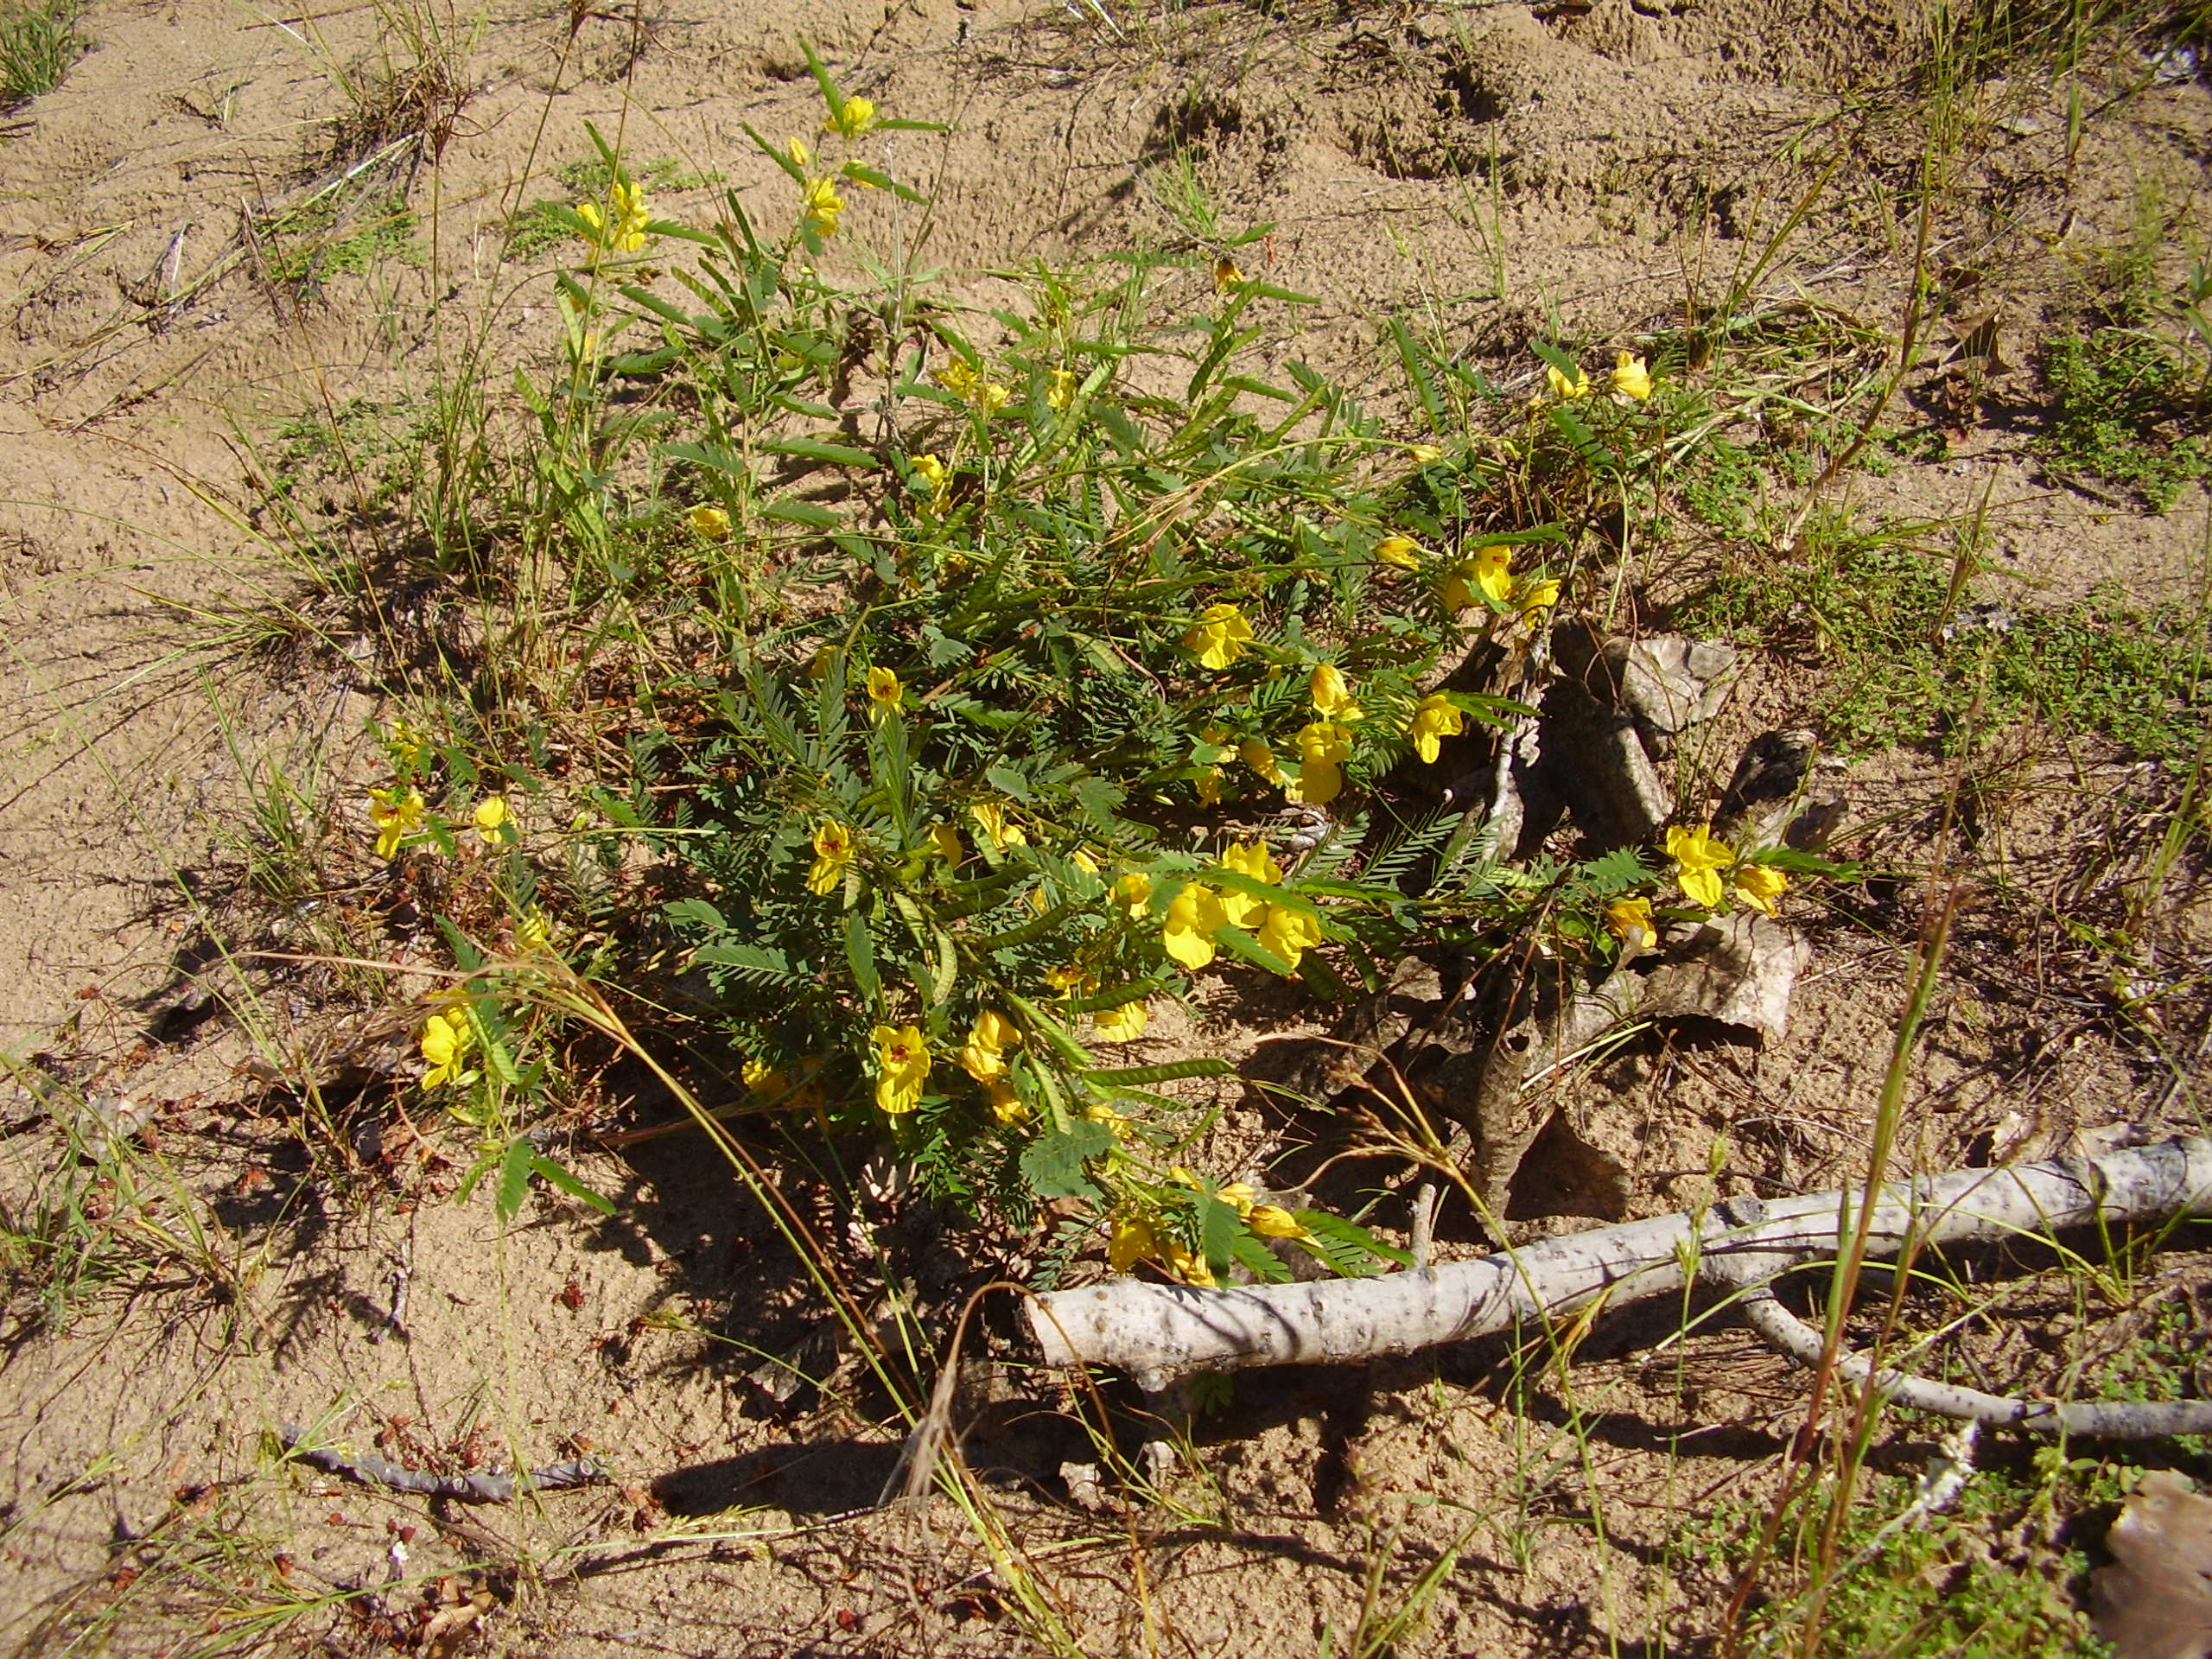
\includegraphics[width=5cm, keepaspectratio]{chamae.png}
		\end{column}
	\begin{column}{5cm}
		\begin{center}
			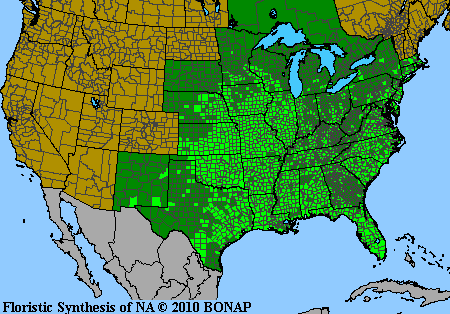
\includegraphics[width=5cm]{chamae_distribution.png}\\
	       \end{center}
    \end{column}
  \end{columns}


	\begin{center}
	
	\end{center}
\end{frame}

\begin{frame}{Fitness variation across the range}
	\begin{center}
		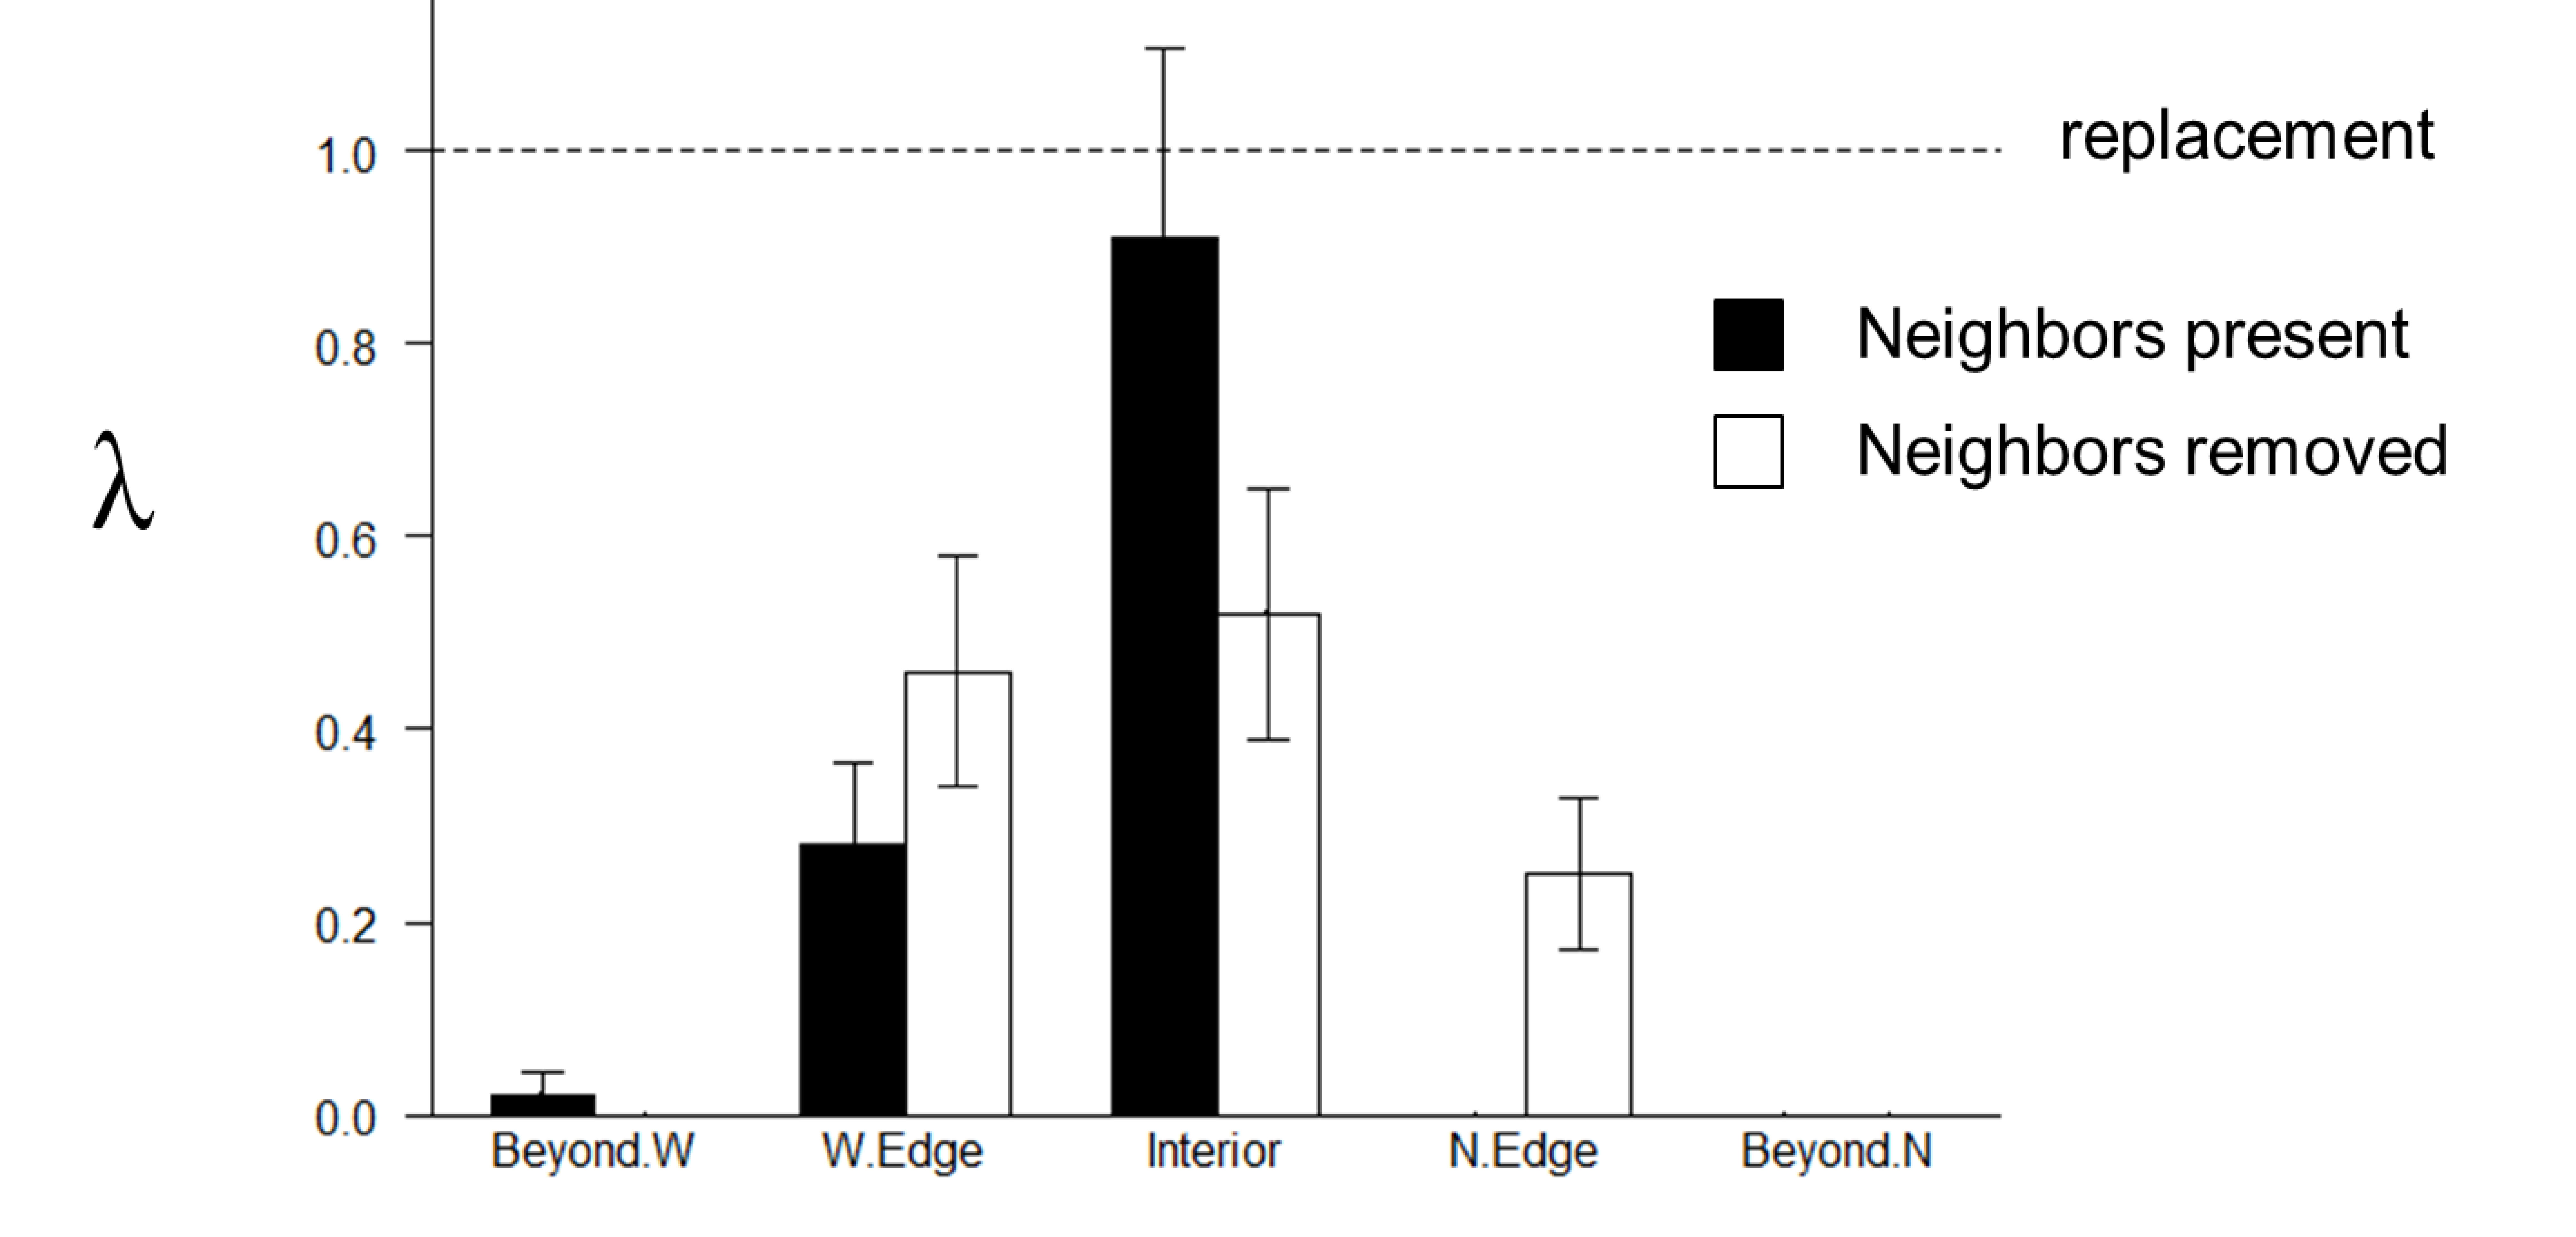
\includegraphics[width=\textwidth, height=\textheight, keepaspectratio]{chamae2010_popgrowth.png}
	\end{center}
	\tiny{Stanton-Geddes et al. 2012 Ecology}
\end{frame}

\begin{frame}{Population history}
	\begin{center}
		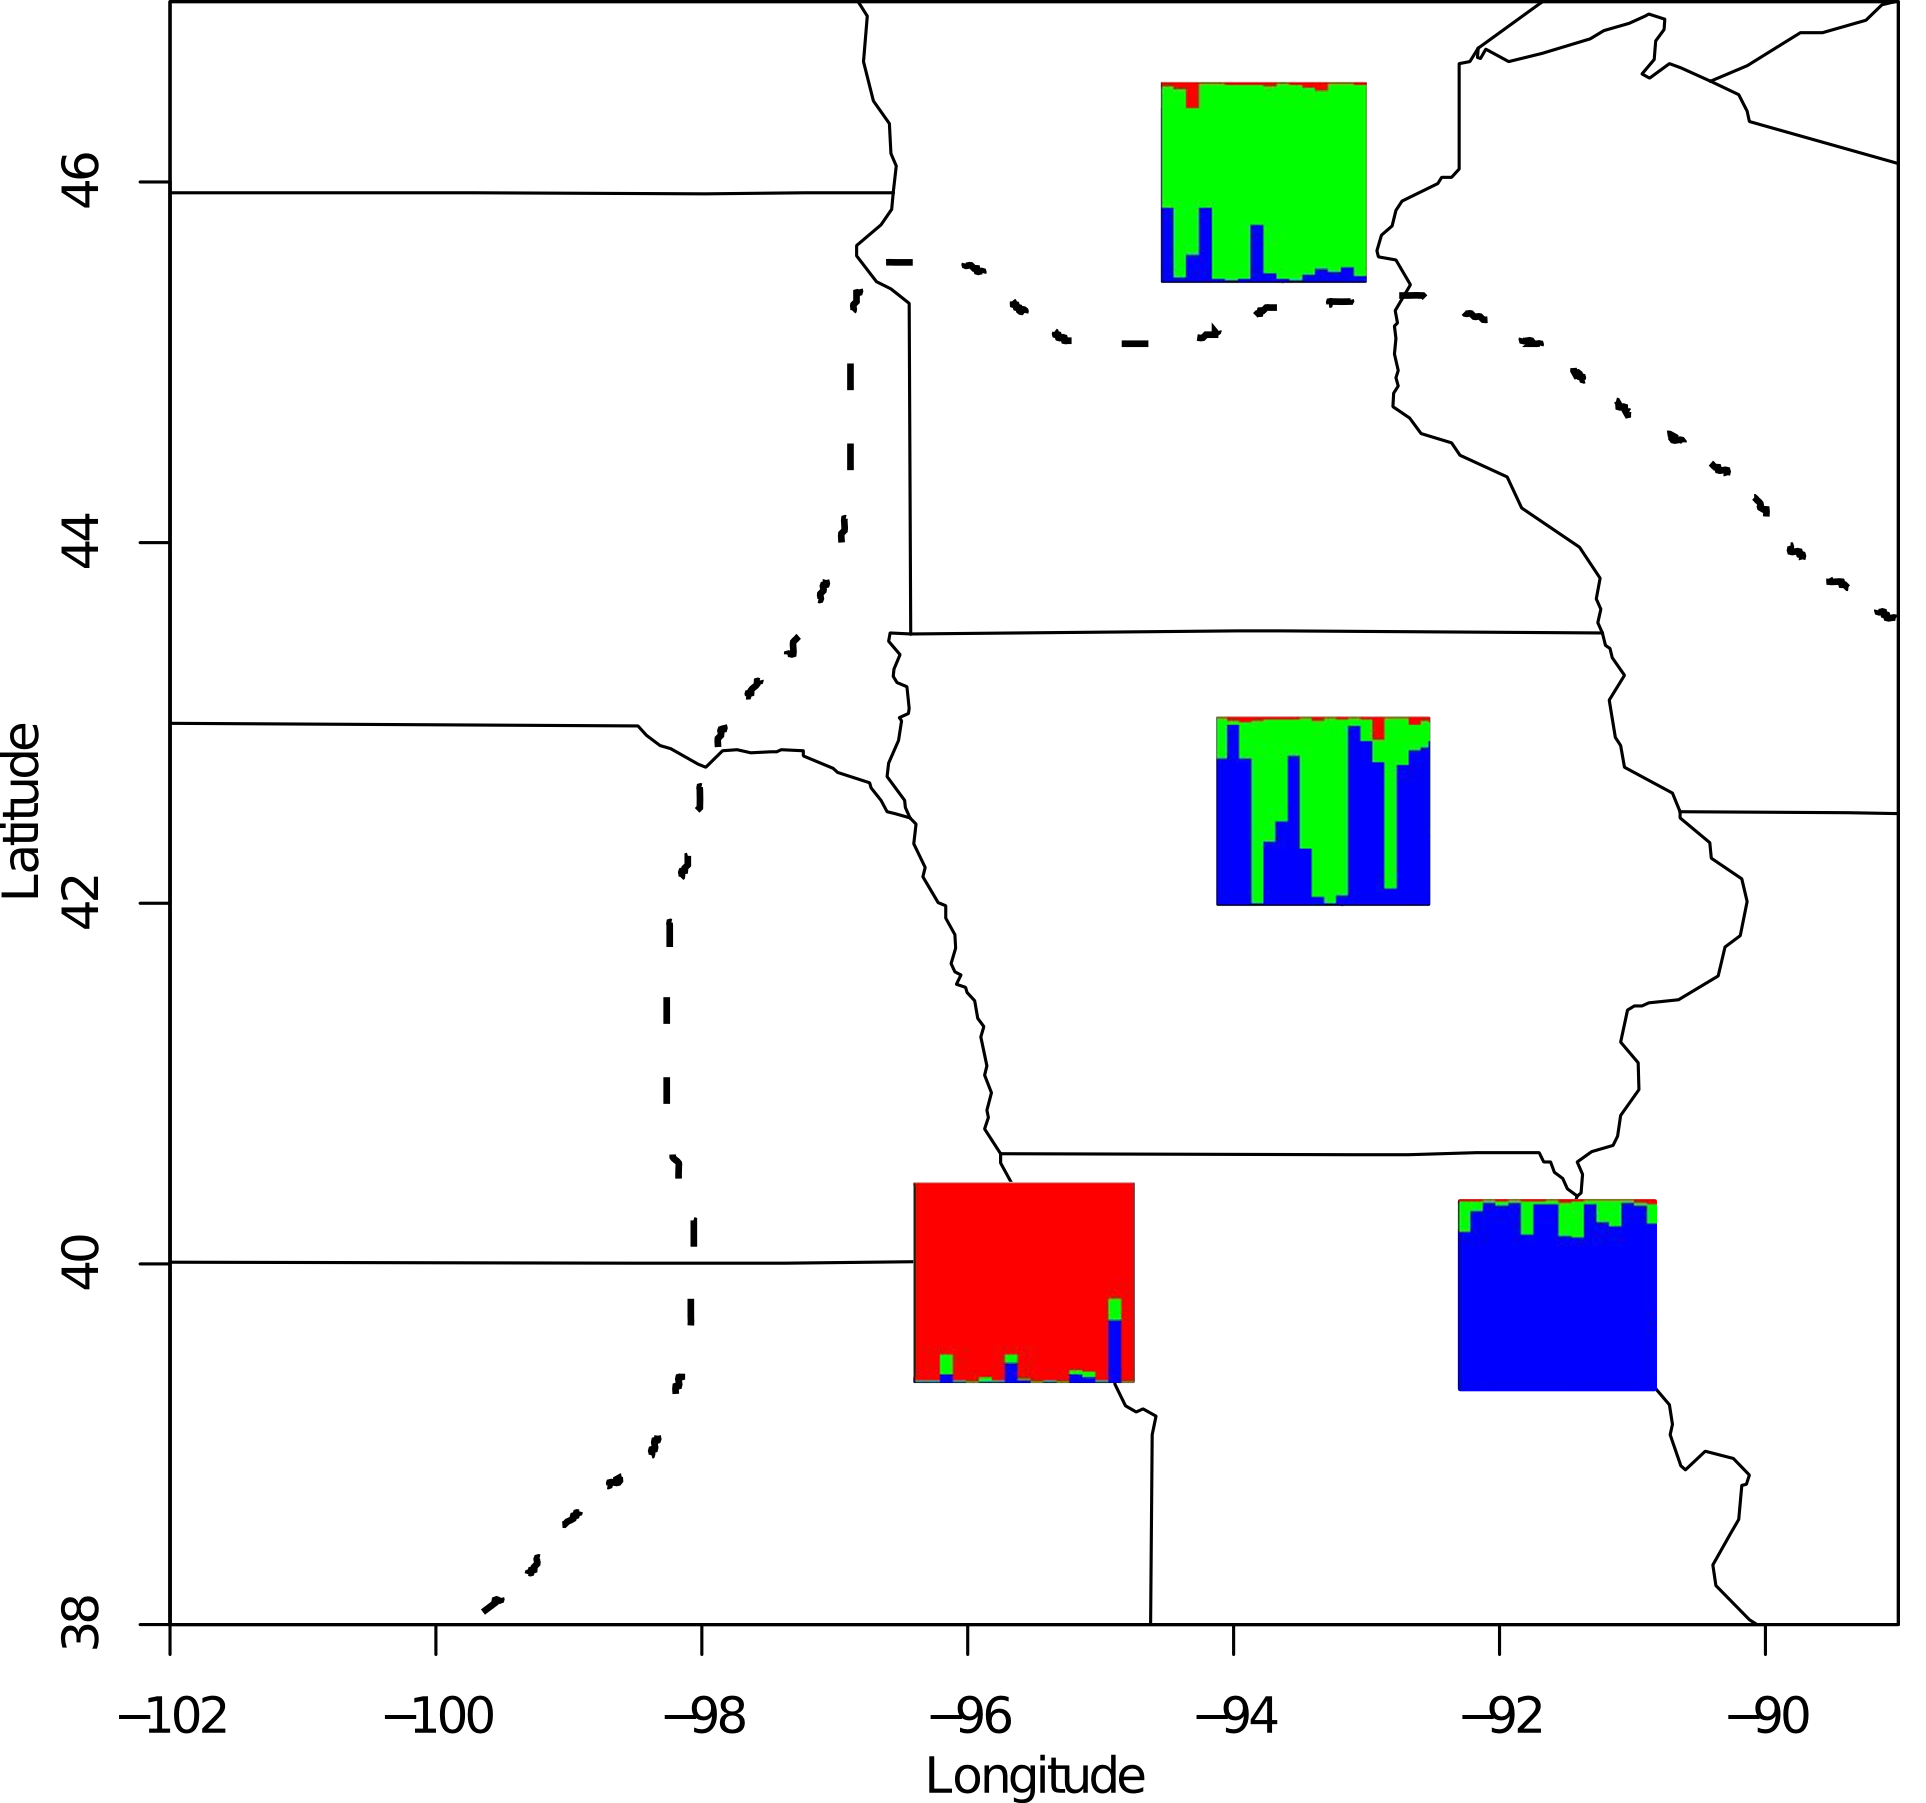
\includegraphics[width=7cm]{chamae_popgen.png}
	\end{center}	
	\tiny{Stanton-Geddes et al. 2013 Am. J. Botany}
\end{frame}

\begin{frame}{Ants}
		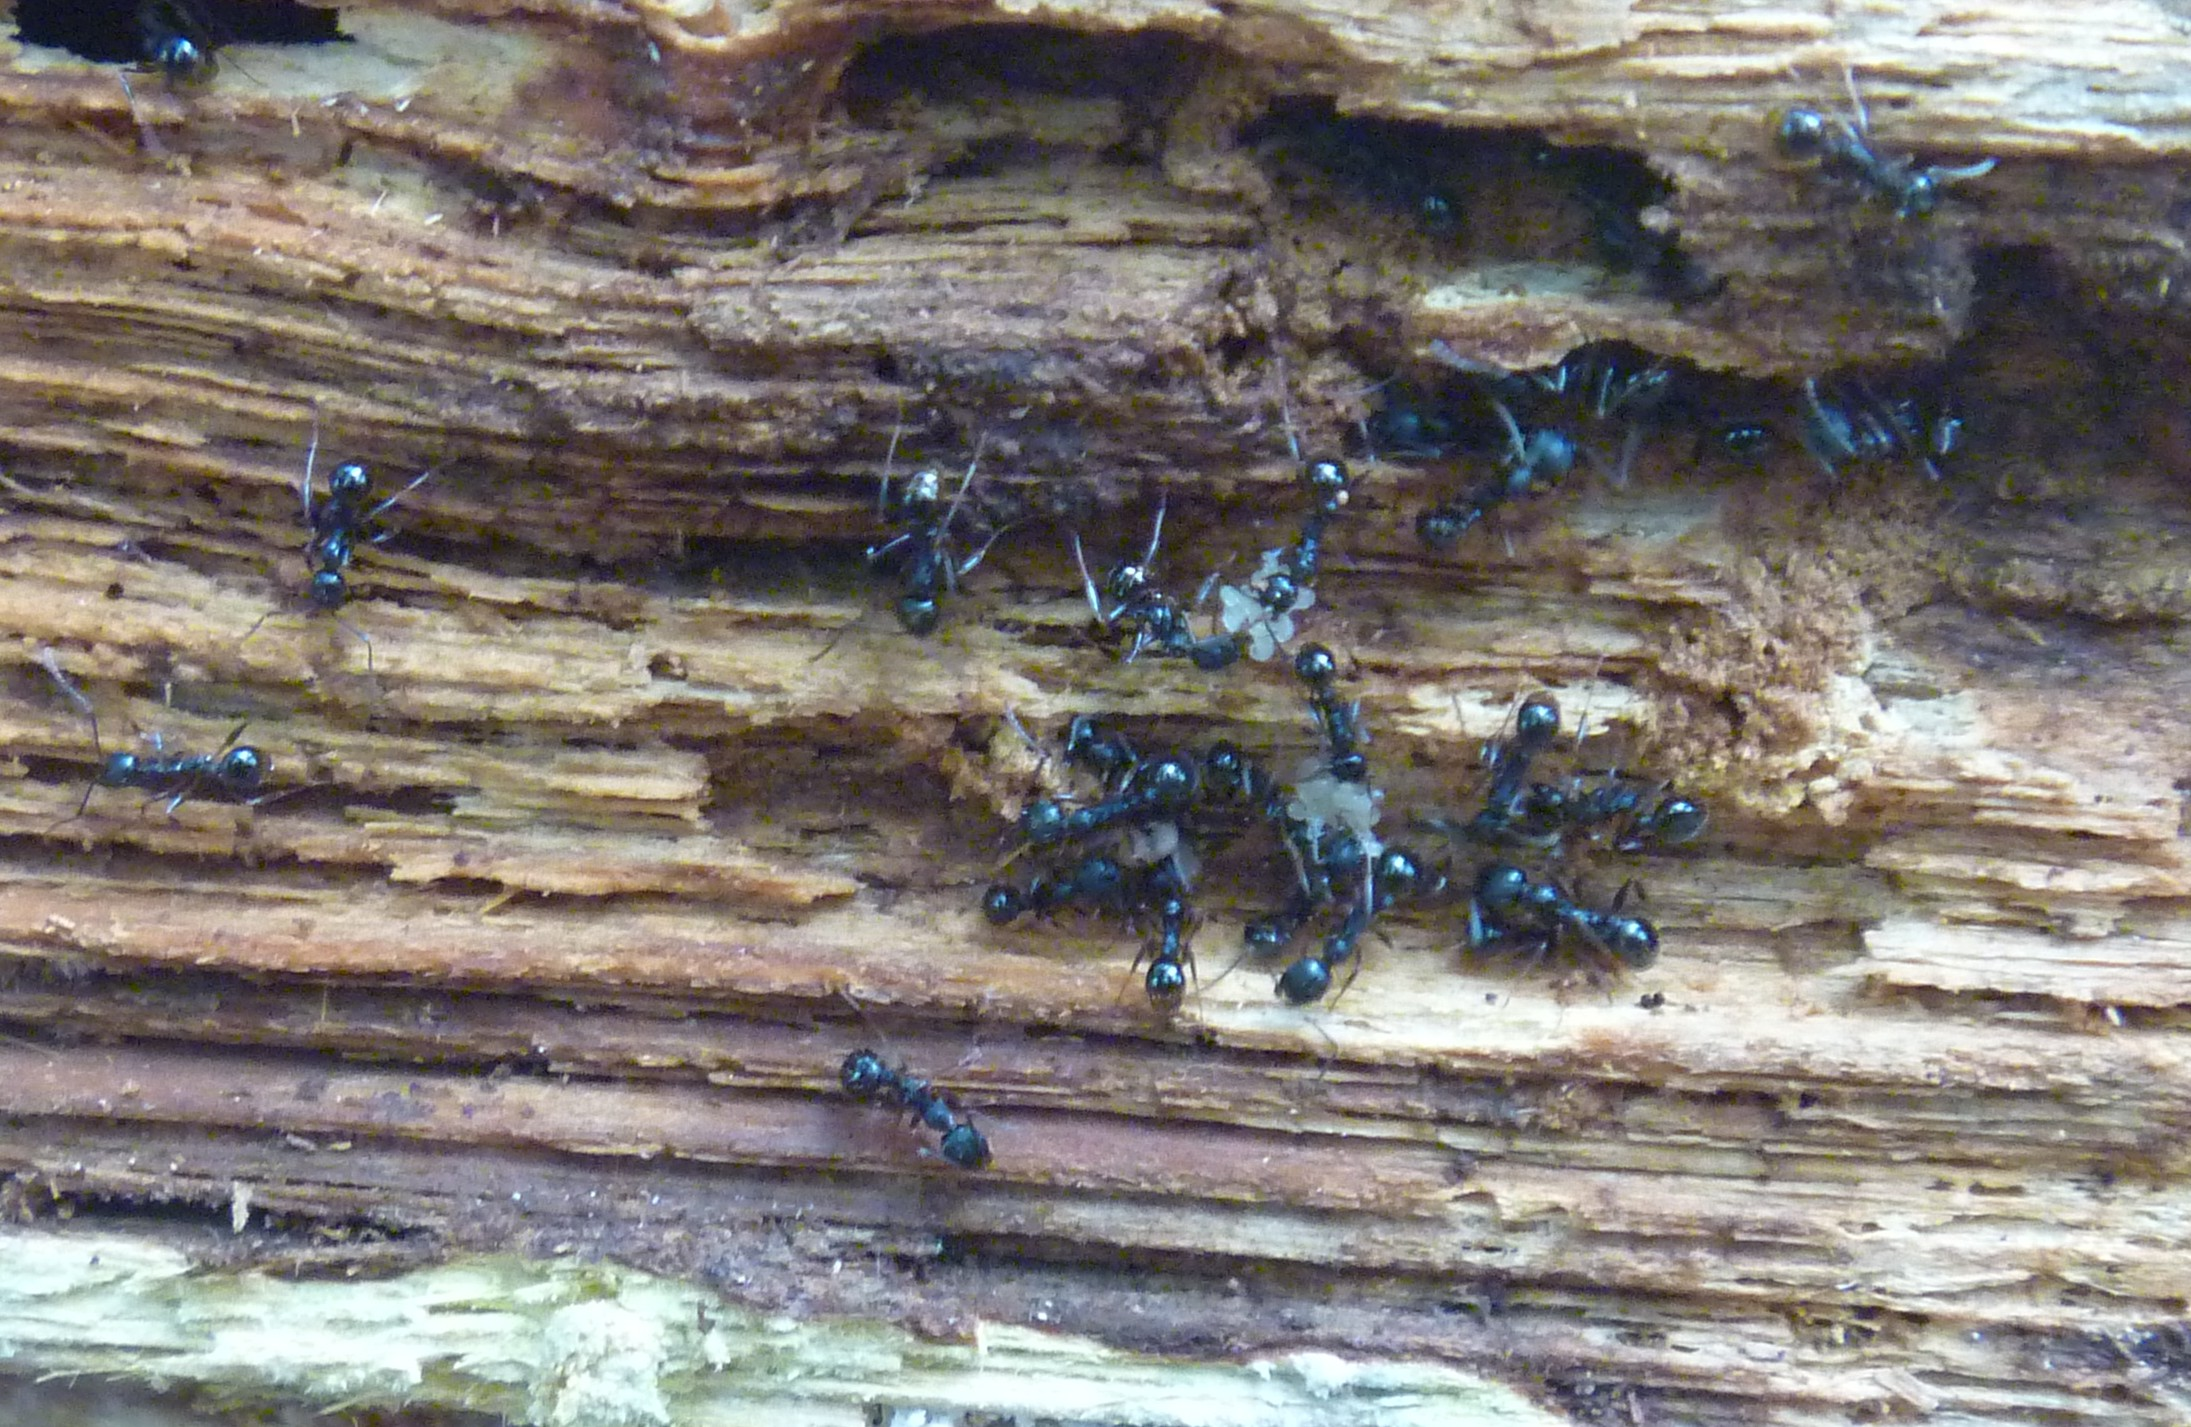
\includegraphics[width=\textwidth, height=\textheight, keepaspectratio]{aphaeno_20130515.png}
\end{frame}

\begin{frame}{Overview}
  \begin{enumerate}
  	\item<1-| alert@1>Progress on the \textit{Aphaenogaster} transcriptome
  	\item Identifying genes associated with thermal tolerance
	\item Latitudinal variation in gene expression
  	\item Population genomics of \textit{Aphaenogaster}
  	\item What is the adaptive potential of \textit{Aphaenogaster} to climate change?
  \end{enumerate}
\end{frame}


\begin{frame}{The \textit{Aphaenogaster }Transcriptome}
	\begin{columns}
		\begin{column}{5cm}
			\begin{itemize}
				\item mRNA transcripts
				\item all genes expressed in an organism
				\item about 5\% of total genome
				\item 16-18,000 genes in sequenced ant genomes (Gadau 2012)
			\end{itemize}
		\end{column}
		\begin{column}{5cm}
			\begin{center}
				\includegraphics<1>[width=5cm]{FactSheet_Transcriptome.pdf}\\
			\end{center}
		\end{column}
	\end{columns}
\end{frame}


\begin{frame}{The \textit{Aphaenogaster }Transcriptome}
	\begin{columns}
		\begin{column}{5cm}
			1) Annotation
			\vspace{.5cm}
			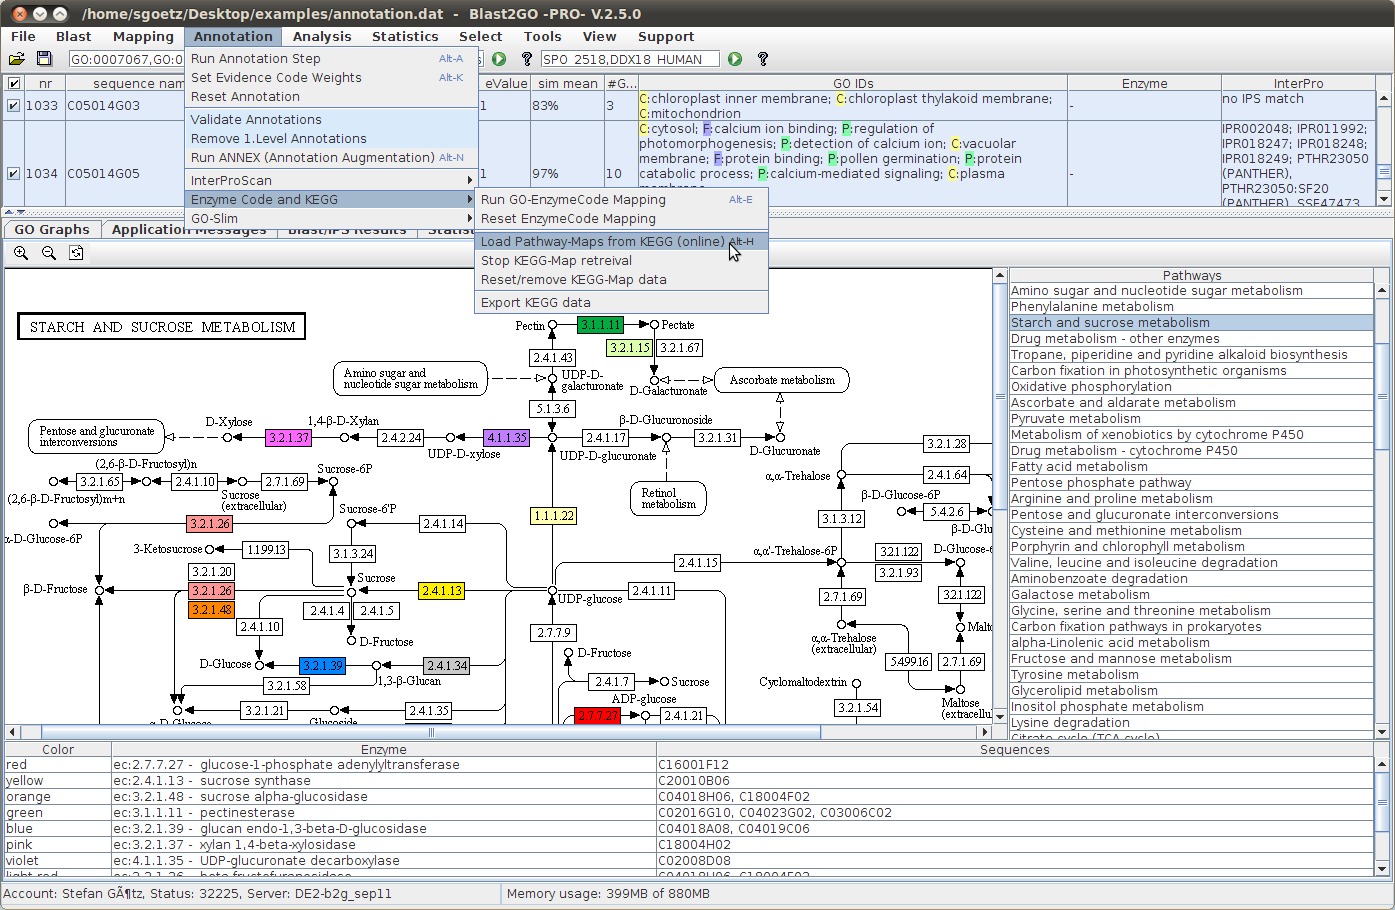
\includegraphics[width=5cm]{BLAST2GO_kegg.png}			

			2) Single nucleotide polymorphisms (SNPs) 		
		\end{column}
		\begin{column}{5cm}
			3) Gene expression
			\vspace{.5cm}
			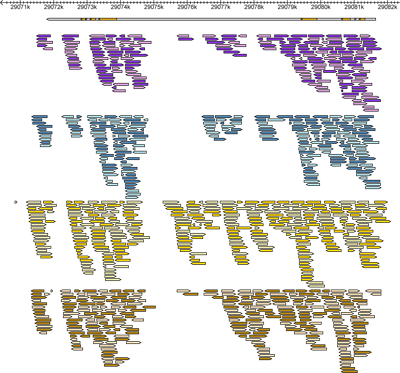
\includegraphics[width=5cm]{rna_seq_bg.png}
		\end{column}
	\end{columns}
\end{frame}


\begin{frame}{Overview}
	\begin{enumerate}
  		\item Progress on the \textit{Aphaenogaster} transcriptome
	  	\item<1-| alert@1> Identifying genes associated with thermal tolerance
		\item Latitudinal variation in gene expression
  		\item Population genomics of \textit{Aphaenogaster}
  		\item What is the adaptive potential of \textit{Aphaenogaster} to climate change?
	\end{enumerate}
\end{frame}


\begin{frame}{Gene Expression}
	\begin{center}
		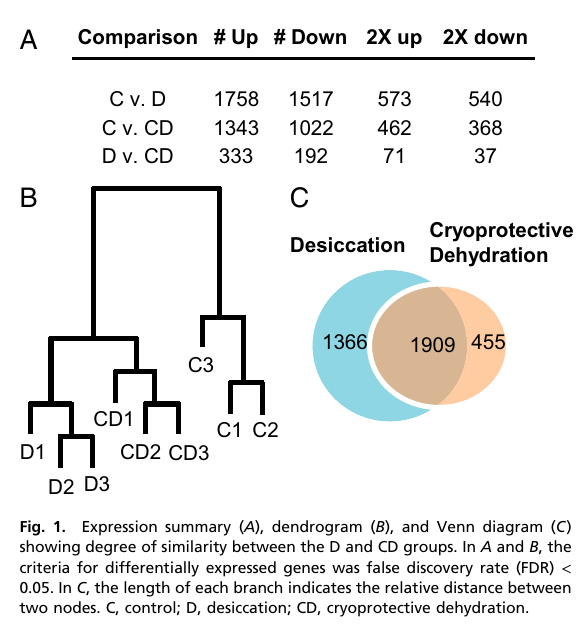
\includegraphics[width=6cm]{Teets2012_Fig1_genex.png}
	\end{center}

	\tiny{Teets et al. 2012 PNAS }
\end{frame}


\begin{frame}{Gene Expression}
	\begin{center}
		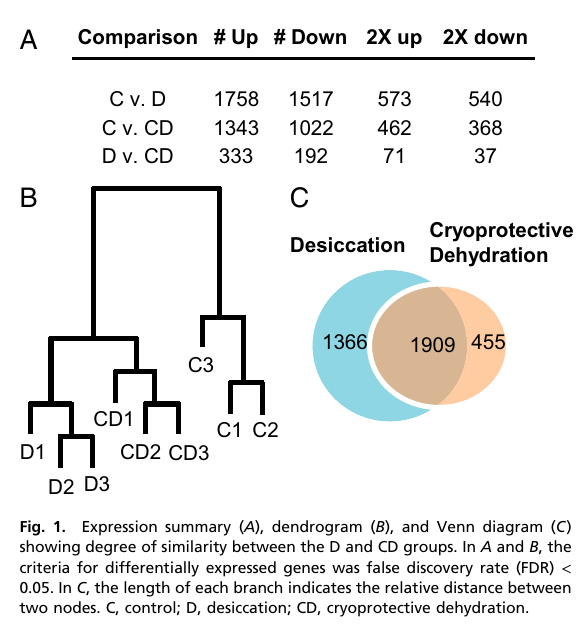
\includegraphics[width=6cm]{Teets2012_Fig1_genex.png}
	\end{center}

	\tiny{Teets et al. 2012 PNAS }
\end{frame}


\begin{frame}{Gene Expression}
	\begin{center}
		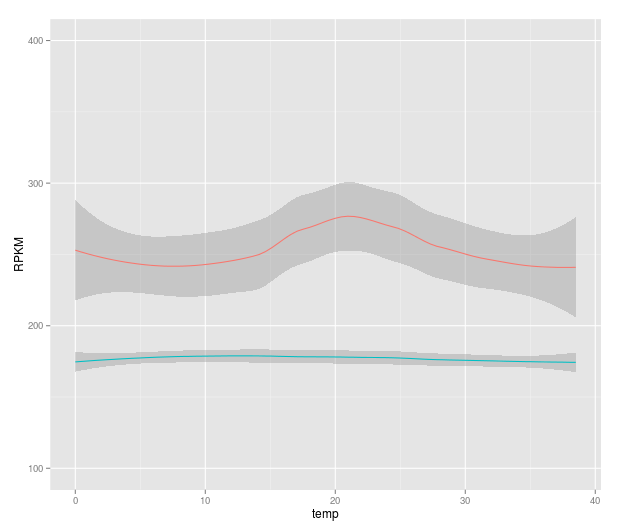
\includegraphics[width=7cm,keepaspectratio]{sim_GenEx_sub.png}
	\end{center}
	\begin{itemize}
		\item Simulated gene expression patterns for two genes
		\item Polynomial based on 12 temperature points (0, 3.5, 7, 10.5, 14, 17.5, 21, 24.5, 28, 31.5, 35, 38.5\degree C)
	\end{itemize}
\end{frame}


\begin{frame}{Gene Expression}
	\begin{block}{Outcomes}
		\begin{enumerate}
			\item Thermal reaction norms for ALL genes
			\item How many genes change expression with temperature?
			\item Do A. picea and A. rudis differ in expression patterns?
			\item Do genes with significant changes in expression have reduced molecular divesity?
		\end{enumerate}
	\end{block}


\end{frame}

\begin{frame}{Overview}
	\begin{enumerate}
  		\item Progress on the \textit{Aphaenogaster} transcriptome
	  	\item Identifying genes associated with thermal tolerance
		\item<1-| alert@1> Latitudinal variation in gene expression
	  	\item<1-| alert@1> Population genomics of \textit{Aphaenogaster}
  		\item What is the adaptive potential of \textit{Aphaenogaster} to climate change?
	  \end{enumerate}
\end{frame}


\begin{frame}{Latitudinal variation in gene expression}
	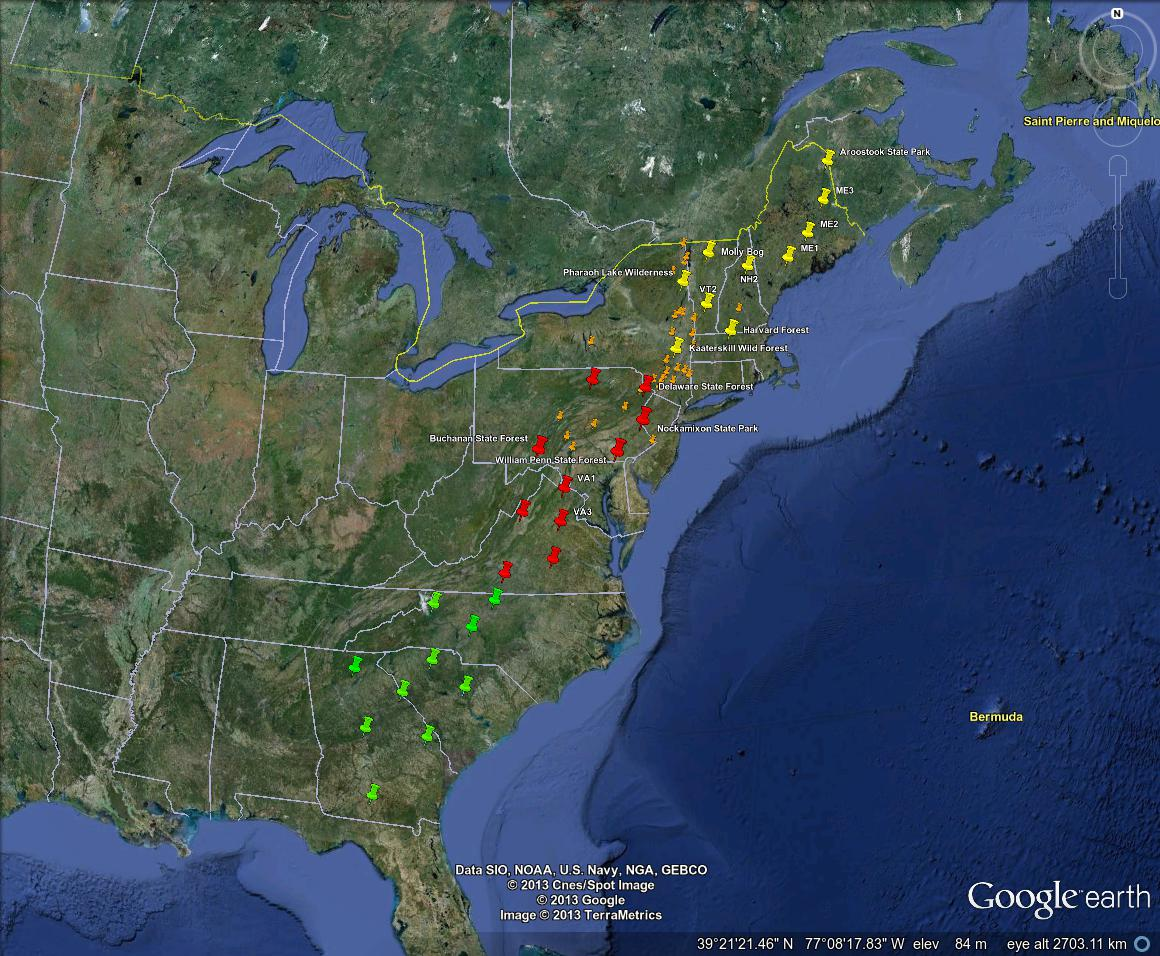
\includegraphics[width=\textwidth, height=\textheight, keepaspectratio]{Aphaenogaster2013_sampling_locations_20130313.jpg}
\end{frame}


\begin{frame}{Latitudinal variation in gene expression}

	\begin{enumerate}
		\item What genes show clinal variation in gene expression?
		\item Are changes in gene expression similar along altitudinal and latitudinal gradients?
	\end{enumerate}
\end{frame}


\begin{frame}{Population genomics of \textit{Aphaenogaster}}
	\begin{columns}
		\begin{column}{5cm}

			SNPs in 3' tail of gene expression tags
			\vspace{1cm}

			\includegraphics<1>[width=5cm]{ovation_DGE.png}\\
		\end{column}
		\begin{column}{5cm}
			\begin{center}
				\begin{itemize}
					\item Do genes with significant changes in expression among sites have reduced molecular diversity? different haplotypes?
					\item How are populations structured?
					\item What is the extent of gene flow? Male vs female dispersal?
				\end{itemize}
			\end{center}
		\end{column}
	\end{columns}
\end{frame}


\begin{frame}{Overview}
	\begin{enumerate}
  		\item Progress on the \textit{Aphaenogaster} transcriptome
	  	\item Identifying genes associated with thermal tolerance
		\item Latitudinal variation in gene expression
	  	\item Population genomics of \textit{Aphaenogaster}
  		\item<1-| alert@1> What is the adaptive potential of \textit{Aphaenogaster} to climate change?
	  \end{enumerate}
\end{frame}


\begin{frame}{Adaptive potential of \textit{Aphaenogaster picea} to warming}
	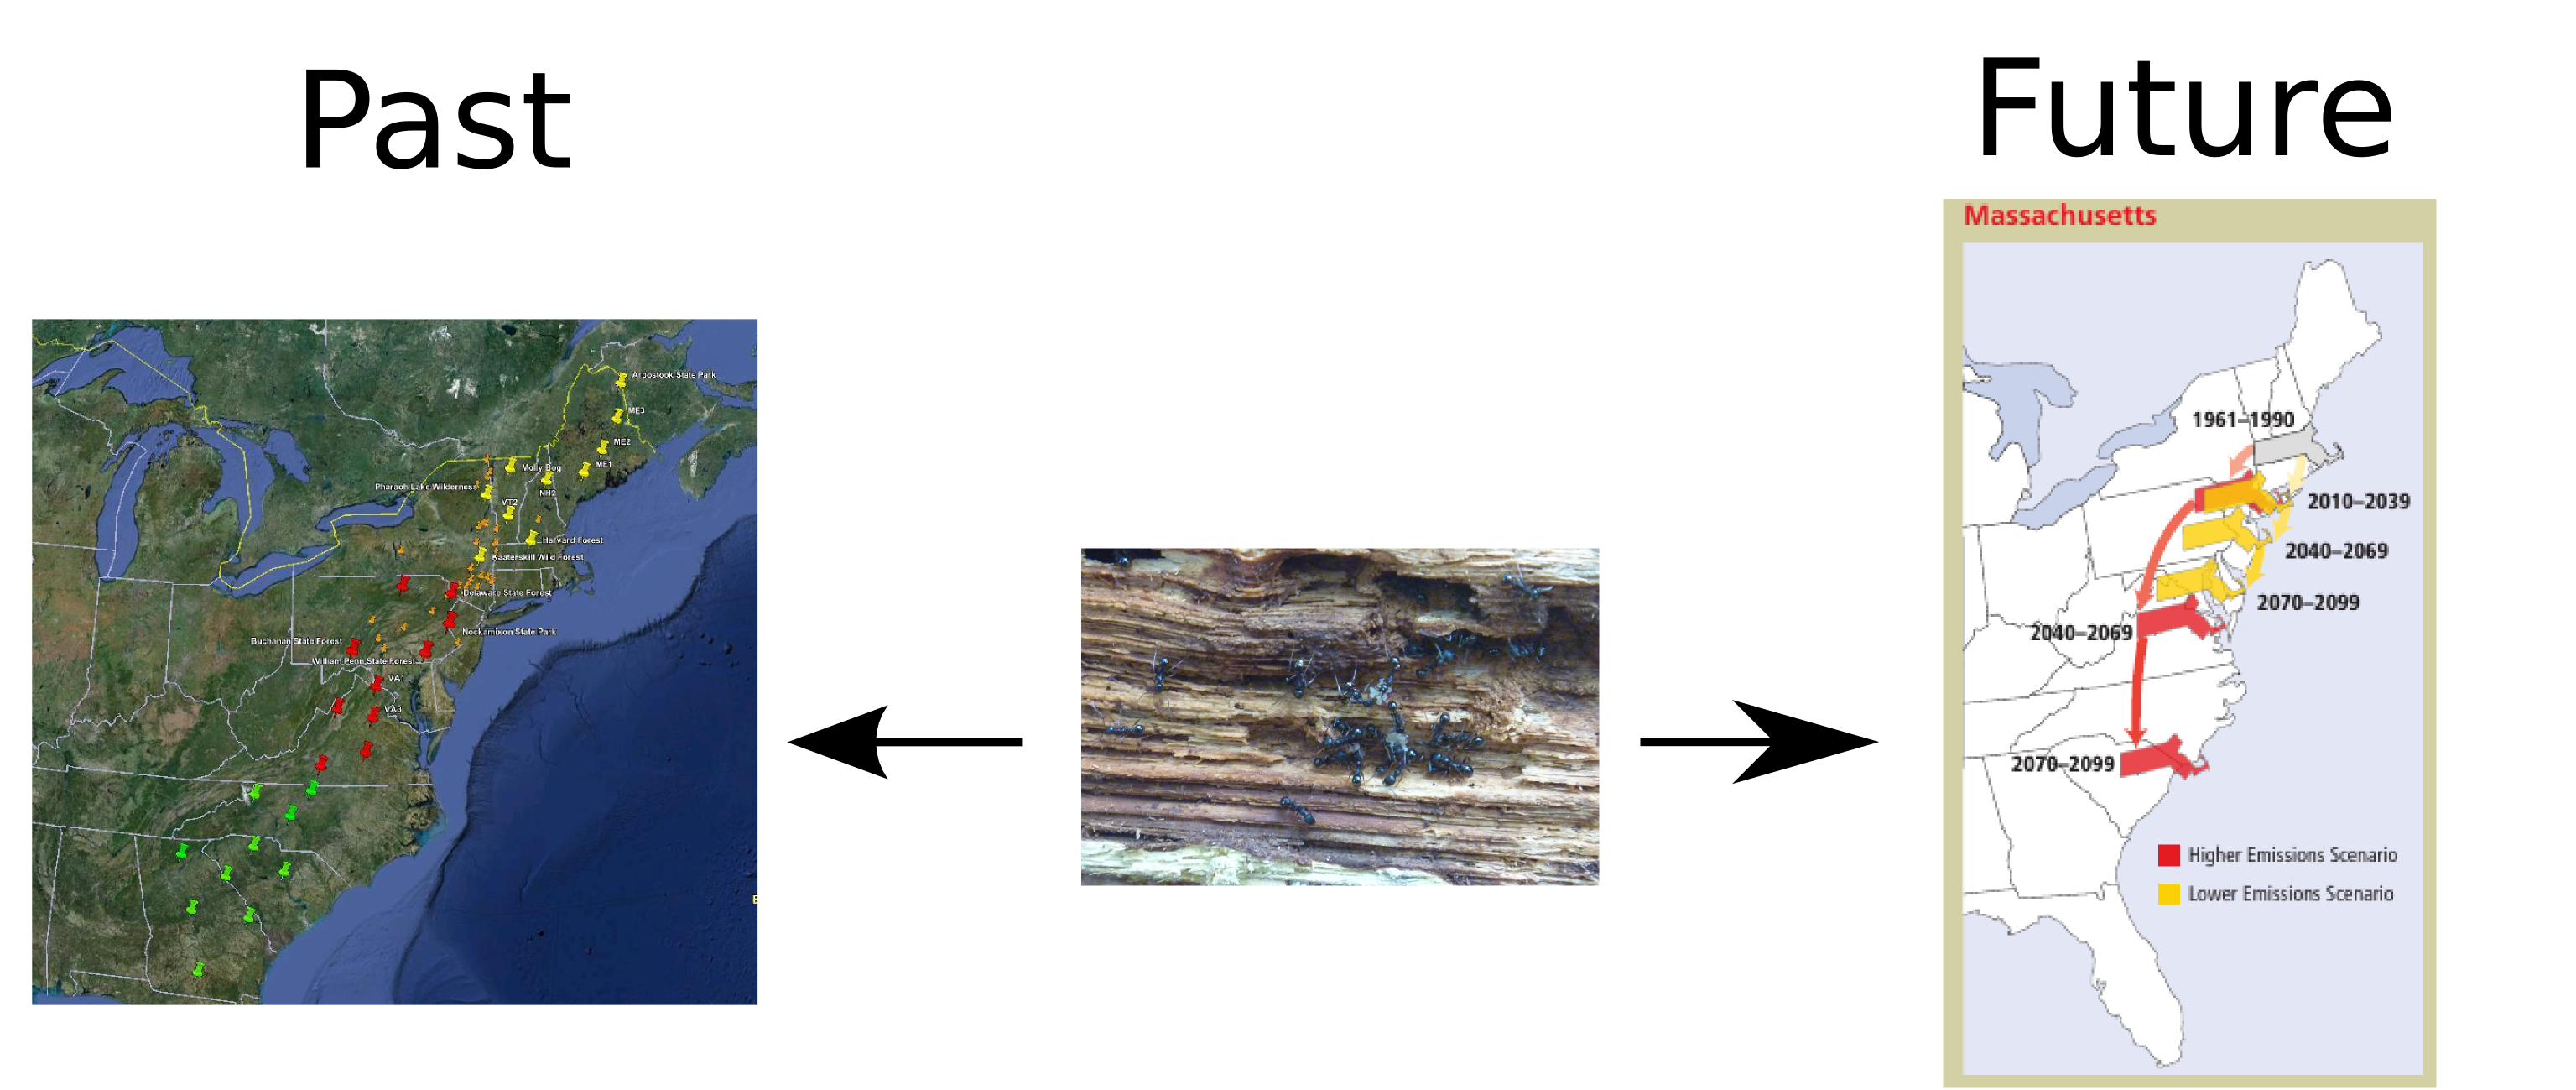
\includegraphics[width=\textwidth, height=\textheight, keepaspectratio]{aphaeno_predictive.png}
\end{frame}

\begin{frame}{Adaptive potential of \textit{Aphaenogaster picea} to warming}

	Given climate predictions, does \textit{Aphaenogaster} have the potential to adapt to climate change \emph{in situ}?	

	\begin{block}{Adaptive potential}
		The \textbf{potential} for species to respond to climate change depends on the \textbf{heritability} (proportion of phenotypic variation that is genetic. 

		$$R = h^2 S$$ \\

		where $$ h ^ 2 $$ is heritability and \textit{S} is the strength of selection 

		\textit{Response} to selection depends on heritability \\

	        $$ H^2 = V_g/V_p $$

	\end{block}
\end{frame}


\begin{frame}{Adaptive potential of \textit{Aphaenogaster picea} to warming}
	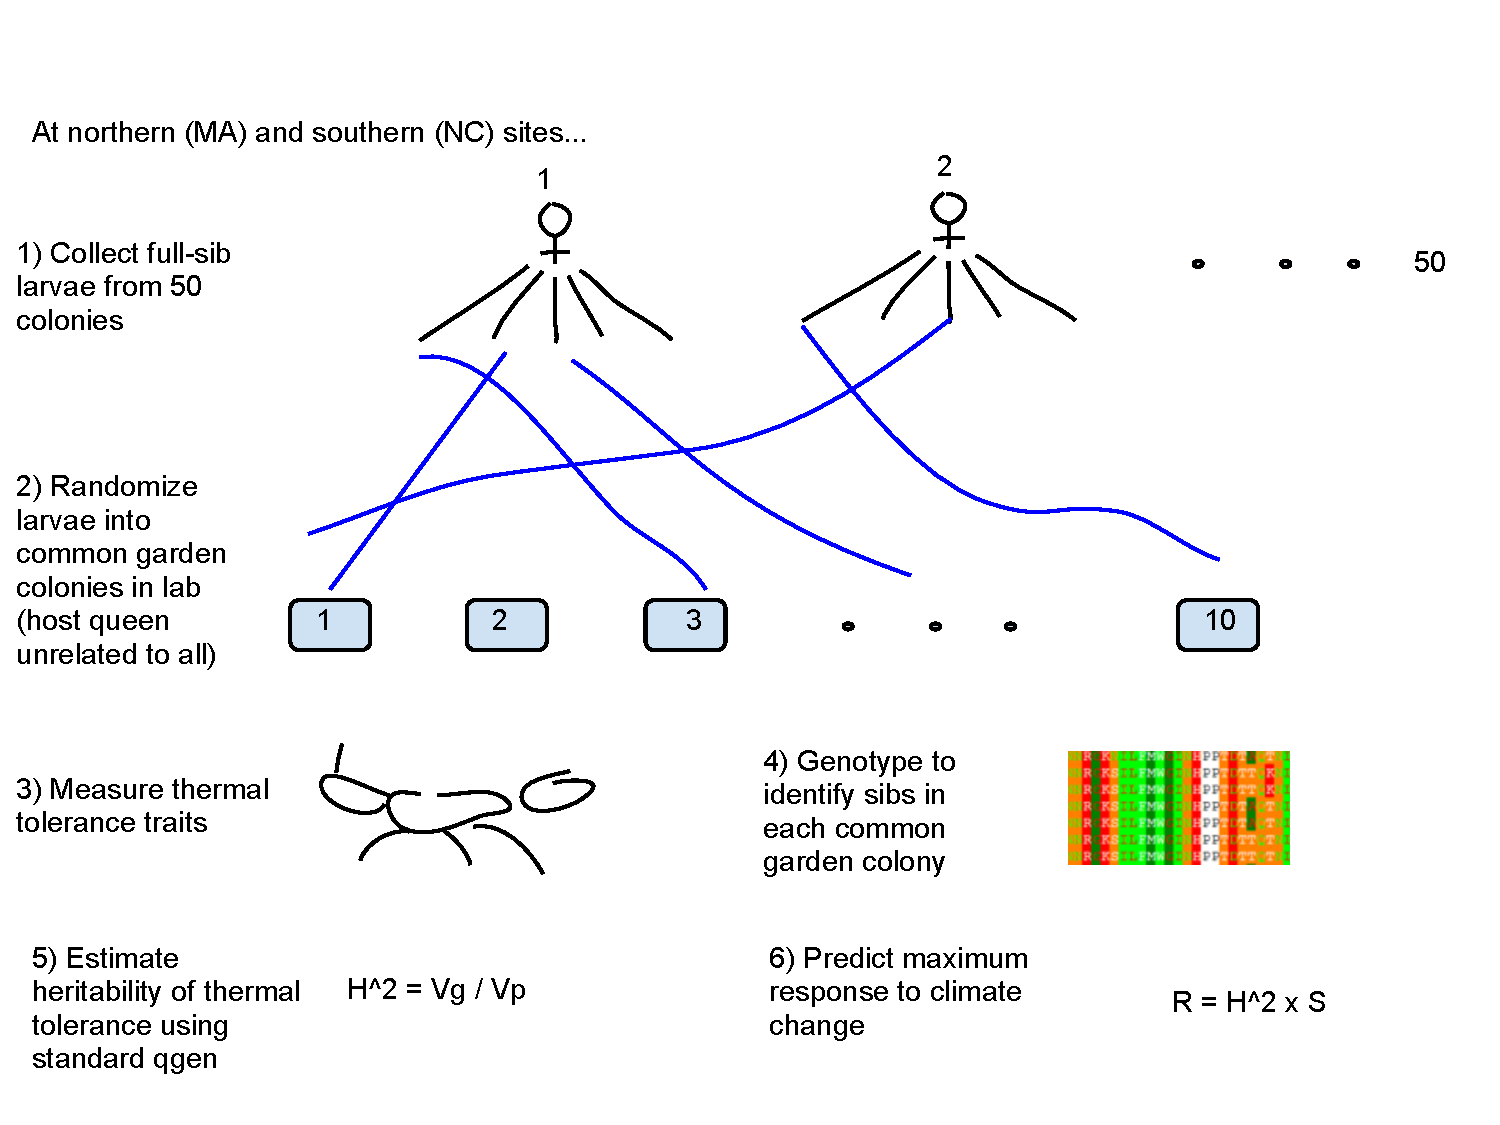
\includegraphics[width=\textwidth, height=\textheight, keepaspectratio]{adaptive_potential_diagram.pdf}
\end{frame}{}


\begin{frame}{ Adaptive potential of \textit{Aphaenogaster picea} to warming}
	\begin{block}{Interpretation of results}
		\begin{itemize}
			\item Is heritability low or high? 
			\item Does heritability differ for cold and heat tolerance?
			\item Genetic correlations between heat and cold tolerance?
			\item Given \textit{h\textsuperscript{2}} can calculate the number of generations required for northern population to match phenotype of southern population...is it adequate to match rate of climate change?
		\end{itemize}

		\tiny{Etterson and Shaw 2000 Science}
	\end{block}
\end{frame}


\begin{frame}{3) Adaptive potential of \textit{Aphaenogaster picea} to warming}
	\textit{Thanks!}
	\begin{itemize}
		\item Sara and Nick
	\end{itemize}

	Tomorrow - sampling protocol!

\end{frame}

\end{document}

